\documentclass{book}[oneside]
\usepackage{CJKutf8}
\usepackage{amsmath}
\usepackage{amsfonts}
\usepackage{amsthm}
\usepackage{titlesec}
\usepackage{titletoc}
\usepackage{xCJKnumb}
\usepackage{clrscode3e}


\usepackage{tikz}
\titleformat{\chapter}{\centering\Huge\bfseries}{第\, \xCJKnumber{\thechapter}\,
    章}{1em}{}
  % \renewcommand{\chaptermark}[1]{\markboth{第 \thechapter 章}{}}
\usepackage{mathrsfs}

\newtheorem{Def}{定义}
\newtheorem{Thm}{定理}
\newtheorem{Cor}{推论}
\newtheorem{Ax}{公理}

\newtheorem{Exercise}{练习}

\newtheorem{Example}{例}


\begin{document}
\begin{CJK*}{UTF8}{gbsn}
  \title{树}
  \author{}
  \date{}
  \maketitle
  % \tableofcontents
  


  \setcounter{chapter}{6}
  \begin{Def}
    连通且无圈的无向图称为无向树,简称{\bfseries树}。 一个没有圈的无向图
    称为无向森林,简称{\bfseries森林}。
  \end{Def}

  \begin{Thm}
  设$G=(V,E)$为一个$(p,q)$图,下列各命题等价:
  \begin{enumerate}
  \item $G$为树;
  \item $G$为连通的且$q = p - 1$;
  \item $G$中无圈且$q = p - 1$。
  \end{enumerate}
\end{Thm}
\begin{proof}[证明]  \mbox{}\par{}

  $1\Rightarrow2$

  (证法一)
  
    只需证$q=p-1$,用数学归纳法证明,施归纳于顶点数$p$。
    
    (1)当$p=1$时,$q=0$,结论显然成立。

    (2)假设当$p=k$时结论成立,往证当$p=k+1$时结论也成立。设树$G$有$k+1$个顶点。$G$中一定存在一个度为1的顶点,这是因为,设$P$为$G$中的一条最长路,$v$为$P$的一个端点,则$v$除了$P$上与其关联的边之外,由$G$中无圈知$v$不能再有其他的与$P$上的顶点相关联的边,同时由$P$为一条最长路知$v$不能再有与$P$外的顶点相关联的边,因此$v$的度必为1。去掉$G$中一个度为1的顶点及其与之关联的边,得到的图$G'$连通且无圈,则$G'$是树。$G'$有$k$个顶点,$q-1$条边,由归纳假设,$q-1 = k - 1$,从而$q = (k +1) - 1$,即当$p=k+1$时结论也成立。

    (证法二)
    
    只需证$q=p-1$,用数学归纳法证明,施归纳于边数$q$。
    
    (1)当$q=0$时,$p=1$,结论显然成立。

    (2)假设当$q<k$时结论成立,往证当$q=k$时结论也成立。设树$G$有$k$条边。去掉$G$中的任意一条边,得到两个支$G_1$和$G_2$,它们均连通无圈,因此是树。设$G_1$有$p_1$个顶点,$k_1$条边,$G_2$有$p_2$个顶点,$k_2$条边,由归纳假设,
    \begin{equation*}
      \begin{split}
        k_1 &= p_1 - 1\\
        k_2 &= p_2 - 1
      \end{split}
    \end{equation*}
    以上两式相加,两边再同时加1,得
    \[k_1 + k_2  + 1 = p_1 + p_2 - 1\]
    从而
    \[k = p - 1 \]
    即当$q=k$时结论也成立。



    $2\Rightarrow3$

只需证$G$中无圈。用反证法。假设图$G$中有圈,则去掉圈上的一条边,得到的图仍然为连通的。如果新得到
的图仍然有圈,在圈上再去掉一条边,又会得到一个新的连通的图。如此继续下去,最终会
得到一个连通的没有圈的图。由从$1$到$2$的证明知最后得到的图中有$p-1$条边,这与去掉
边之前图$G$中的边数$q=p-1$矛盾。


 $3\Rightarrow1$

 只需证$G$连通。设图$G$有$k$个支,则图$G$中的每个支连通且没有圈。设第$i$个支中含有$p_i$个顶点,
$q_i$条边。由$1$到$2$的证明知在第$i$个支中$q_i=p_i-1$。将所有支的边数和顶点数相
加,可得$q = p-k$。于是$k=1$,从而$G$为连通的。
\end{proof}

%\newtheorem*{Exercise}{习题}
\begin{Exercise}
  设$a_1$,$a_2$,$\cdots$,$a_p$为$p$个正整数,$p\geq 2$,并且$\sum_{i=1}^pa_i=2(p-1)$。证明:存在一棵具有$p$个顶点的树,它的各个顶点的度分别为$a_1$,$a_2$,$\cdots$,$a_p$。
\end{Exercise}
\begin{proof}[证明]  用数学归纳法证明,施归纳于$p$。

  (1)当$p=2$时,$a_1+a_2=2(2-1)=2$。由$a_1$,$a_2$为正整数知,$a_1=1$,$a_2=1$。两个顶点之间联结一条边,就构成了一棵满足条件的树。

  (2)假设当$p=k(k\geq 2)$时结论成立,往证当$p=k+1$时结论成立。设$a_1$,$a_2$,$\cdots$,$a_{k+1}$为$k+1$个正整数,并且$\sum_{i=1}^{k+1}a_i=2(k+1-1)=2k$。此时必存在$s$,$1\leq s \leq k+1$,使得$a_s=1$。否则,如果对任意的$i$,$1\leq i \leq k+1$,$a_i\geq 2$,那么$\sum_{i=1}^{k+1}a_i\geq 2(k+1)$,与$\sum_{i=1}^{k+1}a_i=2k$矛盾。不妨设$a_{k+1}=1$。此时必存在$t$,$1\leq t \leq k$,$a_t>1$。否则,$a_1=a_2=\cdots=a_k=1$,于是$\sum_{i=1}^{k+1}a_i=k+1<2k$,矛盾。不妨设$a_k>1$。于是$a_1,a_2,\cdots,a_{k-1},a_{k}-1$为正整数,并且$a_1 + a_2 + \cdots + a_{k-1} + (a_{k}-1) = 2(k-1)$。由归纳假设,存在一棵具有$k$个顶点的树,它的各个顶点的度分别为$a_1$,$a_2$,$\cdots$,$a_{k-1}$,$a_k-1$。在其度为$a_k-1$的顶点上联结一条边和一个顶点,便得到了一个一棵具有$k+1$个顶点的树,它的各个顶点的度分别为$a_1$,$a_2$,$\cdots$,$a_{k+1}$。
\end{proof}

%   \begin{Thm}
%   设$G=(V,E)$为一个$(p,q)$图,下列各命题等价:
%   \begin{enumerate}
%   \item $G$为树;
%   \item $G$的任意两个不同的顶点间有唯一的一条路联结;
%   \item $G$为连通的且去掉任意一条边则得到一个不连通的图;
%   \item $G$为连通的且$q = p - 1$;
%   \item $G$中无圈且$q = p - 1$;
%   \item $G$中无圈且$G$中任意两个不邻接的顶点间加一条边则得到一个含有圈的图。
%   \end{enumerate}
%   \end{Thm}
%   \begin{proof}[证明]

%     $1\Rightarrow2$

%     用反证法。假设图$G$中存在两个顶点$u$和$v$,在它们之间存在两条不同的路$P_1$和
%     $P_2$。由于$P_1\neq P_2$,$P_1$上存在一条边$x=u_1v_1$不在$P_2$上。由$P_1$和
%     $P_2$上所有的顶点和边构成的$G$的子图记为$P_1\cup P_2$, 则$(P_1\cup P_2)- x$
%     是连通的。于是,$(P_1\cup P_2)-x$中存在一条$u_1-v_1$路$P$,$P+x$为$G$的一个
%     圈,矛盾。

%     $2\Rightarrow3$

% 显然,图G为连通的。设$uv$为图$G$的任意一条联结顶点$u$和$v$的边,则$uv$为联结顶点
% $u$和$v$的唯一的一条路,从图$G$中去掉边$uv$之后,顶点$u$和顶点$v$之间没有路,于
% 是得到了一个不连通的图。

% $3\Rightarrow 4$

% 用数学归纳法证明,施归纳于顶点数$p$。

% 当$p=1$时,结论显然成立。

% 假设当$p=k$时结论成立,往证当$p=k+1$时结论也成立。
% 由图$G$为连通的且去掉任意一条边则得到一个不连通的图知图$G$中一定存在一个度为1的
% 顶点$v$。在图$G$中去掉顶点$v$及其与之关联的边,得到图$G'$。则图$G'$为连通的且去
% 掉任意一条边会得到一个不连通的图,由归纳假设,图$G'$中有$k-1$条边,于是图$G$中有
% $k$条边,$q=p-1$成立,定理得证。

% $4\Rightarrow 5$

% 用反证法。假设图$G$中有圈,则去掉圈上的一条边,得到的图仍然为连通的。如果新得到
% 的图仍然有圈,在圈上再去掉一条边,又会得到一个新的连通的图。如此继续下去,最终会
% 得到一个连通的没有圈的图。由从$1$到$4$的证明知最后到的图中有$p-1$条边,这与去掉
% 边之前图$G$中的边数$q=p-1$矛盾。

% $5\Rightarrow 6$

% 设图$G$有$k$个支,则图$G$中的每个支连通且没有圈。设第$i$个支中含有$p_i$个顶点,
% $q_i$条边。由$1$到$4$的证明知在第$i$个支中$q_i=p_i-1$。将所有支的边数和顶点数相
% 加,可得$q = p-k$。于是$k=1$,从而$G$为连通的。设$u$与$v$为图$G$的任意两个不
% 邻接的顶点,则$u$与$v$之间存在一条路,再在$u$与$v$之间加一条边,则得到一个圈。

% $6\Rightarrow 1$

% 设$u$和$v$为图$G$的任意两个顶点。如果$u$和$v$邻接,则$u$和$v$之间有一条路。如果
% $u$和$v$之间不邻接,则在$u$和$v$之间加一条边,会得到一个圈。在该圈上将边$uv$去掉,
% 则得到$u$与$v$之间的一条路。这证明了$G$为连通的。
% \end{proof}
  \begin{Def}
    设$G=(V,E)$为一个图,$G$的一个生成子图$T=(V,F)$如果是树,则称$T$为$G$的{\bfseries 生成树}。
  \end{Def}
  \begin{Thm}
    图$G$有生成树的充分必要条件是$G$为一个连通图。
  \end{Thm}
  \begin{Def}
    设$v$为图$G$的一个顶点,如果$G-v$的支数大于$G$的支数,则称顶点$v$为图$G$的一个{\bfseries 割点}。
  \end{Def}
  \centering
    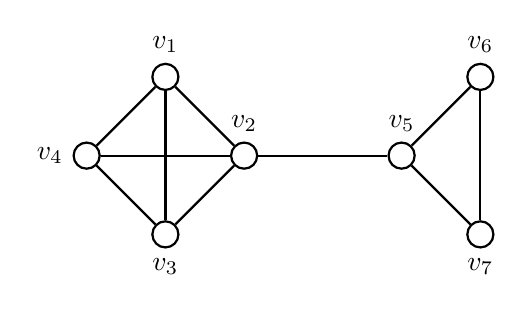
\begin{tikzpicture}[auto,
    specification/.style ={circle, draw, thick}]
   \node[specification] (A) [label=90:$v_1$] at (1,1)  {};
   \node[specification] (B) [label=90:$v_2$] at (2,0)  {};
   \node[specification] (C) [label=-90:$v_3$] at (1,-1)  {};
   \node[specification] (D) [label=180:$v_4$] at (0,0)  {};
   \node[specification] (E) [label=90:$v_5$] at (4,0) {};
   \node[specification] (F) [label=90:$v_6$] at (5,1) {};
   \node[specification] (G) [label=-90:$v_7$] at (5,-1) {};
   \draw[thick] (A) to  (B);
   \draw[thick] (B) to  (C);
   \draw[thick] (C) to  (D);
   \draw[thick] (D) to  (A);
   \draw[thick] (A) to  (C);
   \draw[thick] (B) to  (D);   
   \draw[thick] (B) to  (E);
   \draw[thick] (E) to  (F);
   \draw[thick] (F) to  (G);
   \draw[thick] (G) to  (E);
 \end{tikzpicture}  
  \begin{Thm}
    设$v$为连通图$G=(V,E)$的一个割点,则下列命题等价:
    \begin{enumerate}
    \item $v$为图$G$的一个割点;
    \item 集合$V\setminus \{v\}$有一个二划分$\{U,W\}$, 使得对任意的$u \in U$,$w \in W$,$v$在联结$u$和$w$的每条路上;
    \item 存在与$v$不同的两个顶点$u$和$w$,使得$v$在每一条$u$与$w$间的路上。
    \end{enumerate}
  \end{Thm}
  \centering
    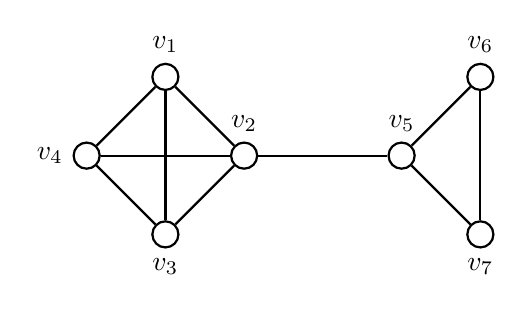
\begin{tikzpicture}[auto,
    specification/.style ={circle, draw, thick}]
   \node[specification] (A) [label=90:$v_1$] at (1,1)  {};
   \node[specification] (B) [label=90:$v_2$] at (2,0)  {};
   \node[specification] (C) [label=-90:$v_3$] at (1,-1)  {};
   \node[specification] (D) [label=180:$v_4$] at (0,0)  {};
   \node[specification] (E) [label=90:$v_5$] at (4,0) {};
   \node[specification] (F) [label=90:$v_6$] at (5,1) {};
   \node[specification] (G) [label=-90:$v_7$] at (5,-1) {};
   \draw[thick] (A) to  (B);
   \draw[thick] (B) to  (C);
   \draw[thick] (C) to  (D);
   \draw[thick] (D) to  (A);
   \draw[thick] (A) to  (C);
   \draw[thick] (B) to  (D);   
   \draw[thick] (B) to  (E);
   \draw[thick] (E) to  (F);
   \draw[thick] (F) to  (G);
   \draw[thick] (G) to  (E);
 \end{tikzpicture}  
  \begin{Def}
   图$G$的一条边$x$称为$G$的一座{\bfseries 桥},如果$G-x$的支数大于$G$的支数。
  \end{Def}
  \centering
    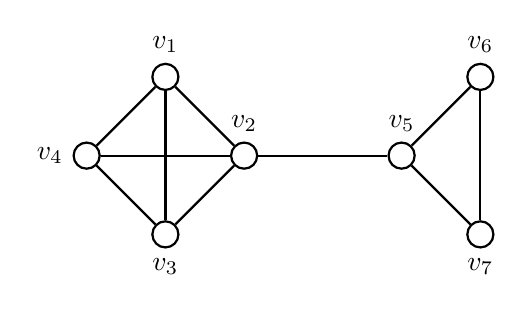
\begin{tikzpicture}[auto,
    specification/.style ={circle, draw, thick}]
   \node[specification] (A) [label=90:$v_1$] at (1,1)  {};
   \node[specification] (B) [label=90:$v_2$] at (2,0)  {};
   \node[specification] (C) [label=-90:$v_3$] at (1,-1)  {};
   \node[specification] (D) [label=180:$v_4$] at (0,0)  {};
   \node[specification] (E) [label=90:$v_5$] at (4,0) {};
   \node[specification] (F) [label=90:$v_6$] at (5,1) {};
   \node[specification] (G) [label=-90:$v_7$] at (5,-1) {};
   \draw[thick] (A) to  (B);
   \draw[thick] (B) to  (C);
   \draw[thick] (C) to  (D);
   \draw[thick] (D) to  (A);
   \draw[thick] (A) to  (C);
   \draw[thick] (B) to  (D);   
   \draw[thick] (B) to  (E);
   \draw[thick] (E) to  (F);
   \draw[thick] (F) to  (G);
   \draw[thick] (G) to  (E);
 \end{tikzpicture}  

   \begin{Thm}
    设$x$为连通图$G=(V,E)$的一条边,则下列命题等价:
    \begin{enumerate}
    \item $x$为$G$的桥;
    \item $x$不在$G$的任一圈上;
    \item 存在$V$的一个划分$\{U,W\}$,使得对任意的$u \in U, w \in W$,$x$在每一条联结$u$与$w$的路上;
    \item 存在$G$的不同顶点$u$和$v$,使得边$x$在联结$u$和$v$的每条路上。
    \end{enumerate}
  \end{Thm}
  \centering
    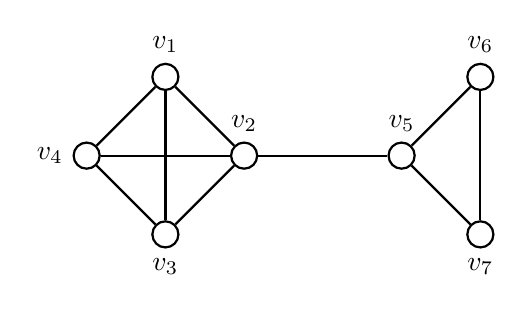
\begin{tikzpicture}[auto,
    specification/.style ={circle, draw, thick}]
   \node[specification] (A) [label=90:$v_1$] at (1,1)  {};
   \node[specification] (B) [label=90:$v_2$] at (2,0)  {};
   \node[specification] (C) [label=-90:$v_3$] at (1,-1)  {};
   \node[specification] (D) [label=180:$v_4$] at (0,0)  {};
   \node[specification] (E) [label=90:$v_5$] at (4,0) {};
   \node[specification] (F) [label=90:$v_6$] at (5,1) {};
   \node[specification] (G) [label=-90:$v_7$] at (5,-1) {};
   \draw[thick] (A) to  (B);
   \draw[thick] (B) to  (C);
   \draw[thick] (C) to  (D);
   \draw[thick] (D) to  (A);
   \draw[thick] (A) to  (C);
   \draw[thick] (B) to  (D);   
   \draw[thick] (B) to  (E);
   \draw[thick] (E) to  (F);
   \draw[thick] (F) to  (G);
   \draw[thick] (G) to  (E);
 \end{tikzpicture}  
  \begin{Def}
    设$G = (V,E)$为图,$S \subseteq E$。如果从$G$中去掉$S$中的所有边得到的图$G-S$的支数大于$G$的支数,而去掉$S$的任一真子集中的边得到的图的支数不大于$G$的支数,则称$S$为$G$的一个{\bfseries 割集}。
  \end{Def}
  \centering
    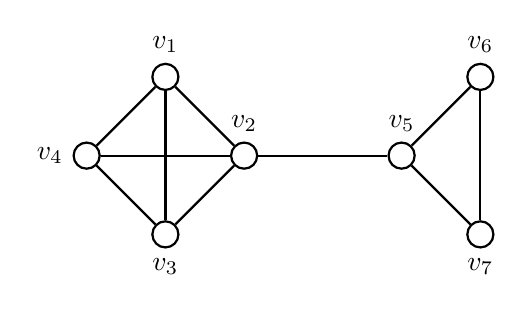
\begin{tikzpicture}[auto,
    specification/.style ={circle, draw, thick}]
   \node[specification] (A) [label=90:$v_1$] at (1,1)  {};
   \node[specification] (B) [label=90:$v_2$] at (2,0)  {};
   \node[specification] (C) [label=-90:$v_3$] at (1,-1)  {};
   \node[specification] (D) [label=180:$v_4$] at (0,0)  {};
   \node[specification] (E) [label=90:$v_5$] at (4,0) {};
   \node[specification] (F) [label=90:$v_6$] at (5,1) {};
   \node[specification] (G) [label=-90:$v_7$] at (5,-1) {};
   \draw[thick] (A) to  (B);
   \draw[thick] (B) to  (C);
   \draw[thick] (C) to  (D);
   \draw[thick] (D) to  (A);
   \draw[thick] (A) to  (C);
   \draw[thick] (B) to  (D);   
   \draw[thick] (B) to  (E);
   \draw[thick] (E) to  (F);
   \draw[thick] (F) to  (G);
   \draw[thick] (G) to  (E);
 \end{tikzpicture}  

  \begin{Exercise}
    恰有两个顶点不是割点的连通图是一条路。
  \end{Exercise}
  \begin{proof}[证明]设连通图$G$有$p$个顶点,恰有两个顶点不是割点,往证$G$为一条路。由$G$连通知,$G$有一棵生成树$T$。取树$T$的一条最长路$P:v_1v_2\cdots v_k$,则$v_1$和$v_k$ 在$T$中的度必为$1$,它们都不是$T$的割点,从而也不是图$G$的割点。由$G$中恰有两个顶点不是割点知,$T$中除了$v_1$和$v_k$之外没有其他度为$1$的顶点,由此可得出$T$中所有顶点的度小于等于$2$。否则,假设$T$中存在一个度大于等于$3$的顶点,则$T$中所有顶点的度数之和$\geq 3 + 2 + 2(p-3) = 2p -1 > 2(p-1)$,矛盾。由$T$中所有顶点的度小于等于$2$知,路$P$中包含了$T$中所有的顶点,即路$P$中包含了$G$中所有的顶点。事实上,$G$就是路$P$。否则,在路$P$中,设$v_i$和$v_j$($j>i+1$)之间在$G$中有一条边,则$v_{i+1}$不是$G$的割点,与$G$中只有两个顶点$v_1$和$v_k$不是割点矛盾。
  \end{proof}

\chapter{}

\end{CJK*}
\end{document}





%%% Local Variables:
%%% mode: latex
%%% TeX-master: t
%%% End:



